\subsubsection{\roofunit}
%
The {\roofunit} gadgets consist of two parts, the scaffolding and the shingles.
%
The scaffolding is responsible for assembling a path from the top of the final most significant digit and adding some height last row.
%
Since the most significant digit is positioned at a different height within a digit region depending on how many digits
are in the MSR, the {\roofscaffolding} gadget's height must take this into consideration.
%
If the MSR has 3 digits, the height is $30$ tiles.
%
If the MSR has 2 digits, the height is $60 + 4l$ tiles.
%
Otherwise, if the MSR has 1 digit the height is $90 + 8l$ tiles.
%



\begin{itemize}
    \item If case 1: create
    $\begin{aligned}[t]
        \roofscaffolding(& \left\langle {\tt RoofScaffolding}, 1, {\tt halt}, {\tt msr}, {\tt msd} \right\rangle,
                           \left\langle {\tt RoofShingle},     0                                   \right\rangle \;)
    \end{aligned}$\\from the gadget shown in Figure~\ref{fig:roof_unit_1}.
    %
    In this step, $90 + 8l + 1 =$
    %
    $91 + 8l =$
    %
    $91 + 8 \cdot \left( \ceil*{\log m} + 2 \right) \leq$
    %
    $91 + 8 \cdot \left( {\log m} + 3 \right) =$
    %
    $115 + 8 \cdot {\log m} = \bigologm$ tiles were created.
    %
    \vspace{0.5cm}

    \item If case 2: create
    $\begin{aligned}[t]
        \roofscaffolding(& \left\langle {\tt RoofScaffolding}, 2, {\tt halt}, {\tt msr}, {\tt msd} \right\rangle,
                           \left\langle {\tt RoofShingle},     0                                   \right\rangle \;)
    \end{aligned}$\\from the gadget shown in Figure~\ref{fig:roof_unit_2}.
    %
    In this step, $60 + 4l + 3$
    %
    $63 + 4l =$
    %
    $63 + 4 \cdot \left( \ceil*{\log m} + 2 \right) \leq$
    %
    $63 + 4 \cdot \left( {\log m} + 3 \right) =$
    %
    $75 + 4 \cdot {\log m} = \bigologm$ tiles were created.
    %
    \vspace{0.5cm}

    \item If case 3: create
    $\begin{aligned}[t]
        \roofscaffolding(& \left\langle {\tt RoofScaffolding}, 3, {\tt halt}, {\tt msr}, {\tt msd} \right\rangle,
                           \left\langle {\tt RoofShingle},     0                                   \right\rangle \;)
    \end{aligned}$\\from the gadget shown in Figure~\ref{fig:roof_unit_3}.
    %
    In this step, $30 + 5 = 35 = O\left( 1 \right)$ tiles were created.
    \vspace{0.5cm}


    \item For each $i = 0,\ldots,g$, create
    $\begin{aligned}[t]
        \roofshingle(& \left\langle {\tt RoofShingle}, i     \right\rangle,
                       \left\langle {\tt RoofShingle}, i + 1 \right\rangle \;)
    \end{aligned}$\\from the gadget shown in Figure~\ref{fig:roof_unit_right_shingles}.
    %
    In this step, $6g \leq$
    %
    $6 \frac{d}{3} =$
    %
    $2d =$
    %
    $O\left( d \right) =$
    %
    $O\left( k \right) =$
    %
    $O\left( {\log N} \right)$ tiles were created.
    %
    \vspace{0.5cm}

    \item If $k$ is odd, we add one additional tile to the rightmost shingle, with a west glue labeled\\ $\left\langle {\tt RoofShingle}, \ceil*{\frac{d}{3}} \right\rangle$.
    In this step $1 = O(1)$ tile was created.

\end{itemize}


\begin{figure}[H]
    \centering
    \subcaptionbox{
        Case 1 - roof unit scaffolding. There are $91 + 8l$ tiles in this gadget.
        \label{fig:roof_unit_1}
    }{\makebox[0.24\textwidth][c]{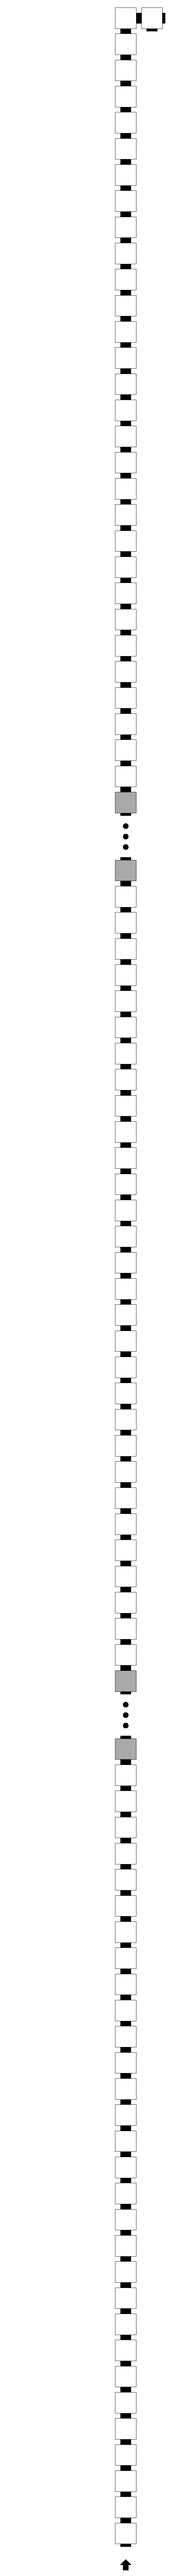
\includegraphics[width=0.45in]{roof_unit_1}}}%
    ~
    \subcaptionbox{
        Case 2 - roof unit scaffolding. There are $63 + 4l$ tiles in this gadget.
        \label{fig:roof_unit_2}
    }{\makebox[0.24\textwidth][c]{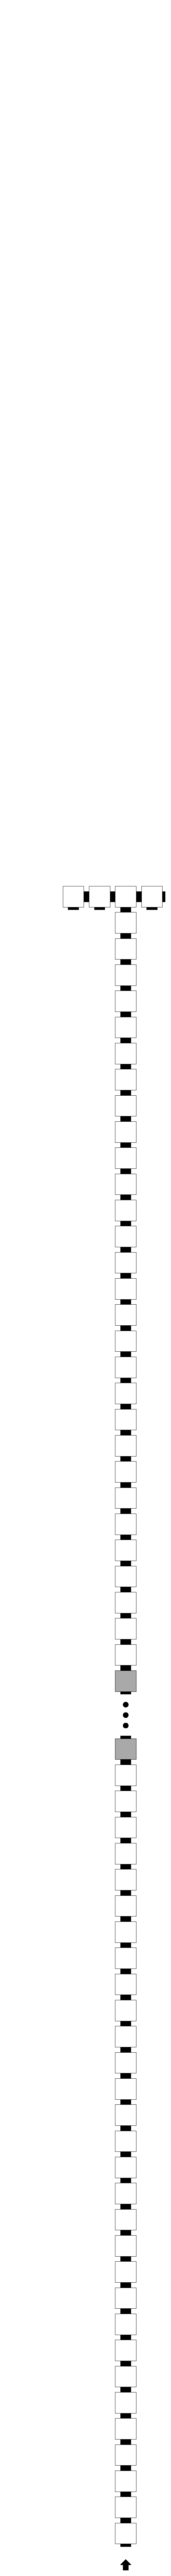
\includegraphics[width=0.45in]{roof_unit_2}}}%
    ~
    \subcaptionbox{
        Case 3 - roof unit scaffolding. There are $35$ tiles in this gadget.
        \label{fig:roof_unit_3}
    }{\makebox[0.24\textwidth][c]{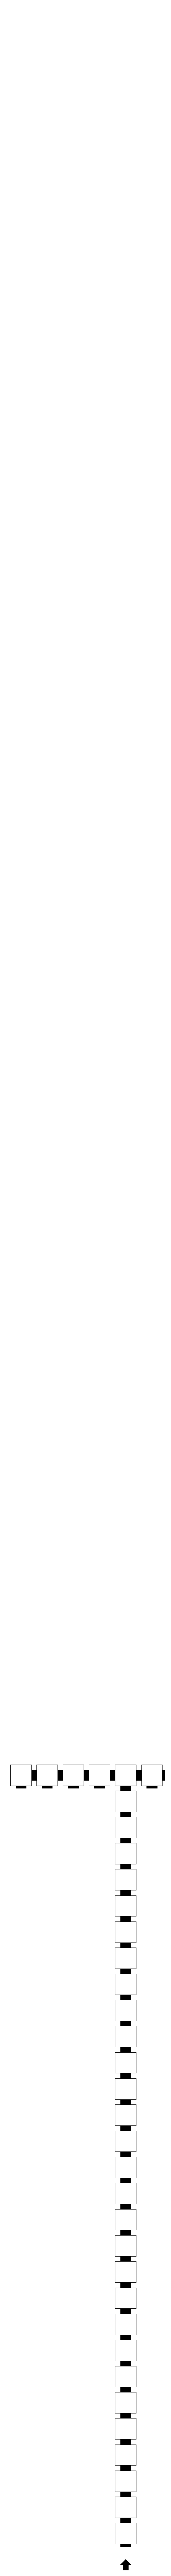
\includegraphics[width=0.45in]{roof_unit_3}}}%
    ~
    \subcaptionbox{
        Right shingles. There are $6$ tiles in this gadget.
        \label{fig:roof_unit_right_shingles}
    }{\makebox[0.24\textwidth][c]{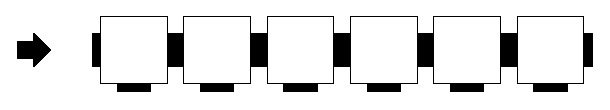
\includegraphics[width=0.45in]{roof_unit_right_shingle}}}%
    ~
\end{figure}
\begin{figure}[H]\ContinuedFloat
    \centering
    \subcaptionbox{
        Case 1  - overview.
        The black tiles in this figure correspond to the gadget shown in subfigure~\subref{fig:roof_unit_1}.
        \label{fig:roof_unit_1_msr_msd_overview}
    }{\makebox[0.32\textwidth][c]{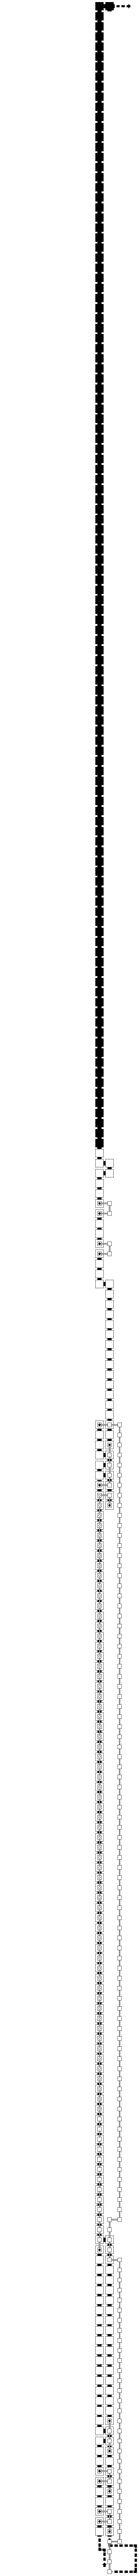
\includegraphics[width=0.45in]{overviews/case1/roof_unit_1_op_msr_msd}}}%
    ~
    \subcaptionbox{
        Case 2 - overview.
        The black tiles in this figure correspond to the gadget shown in subfigure~\subref{fig:roof_unit_2}.
        \label{fig:roof_unit_2_op_msr_msd_overview}
    }{\makebox[0.32\textwidth][c]{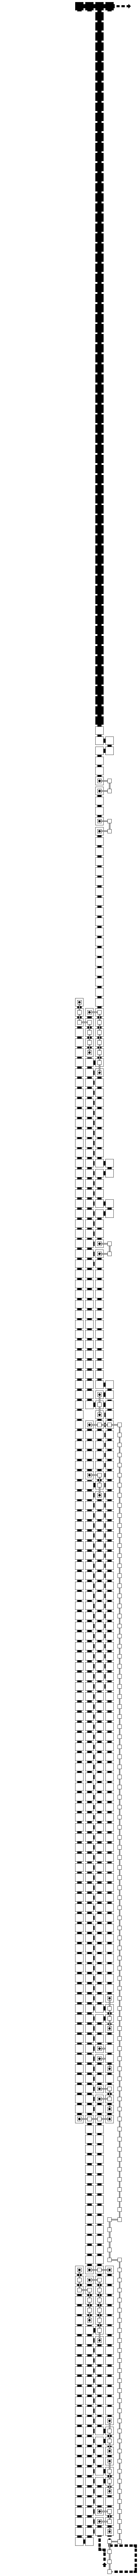
\includegraphics[width=0.45in]{overviews/case2/roof_unit_2_op_msr_msd}}}%
    ~
    \subcaptionbox{
        Case 3 - overview.
        The black tiles in this figure correspond to the gadget shown in subfigure~\subref{fig:roof_unit_3}.
        \label{fig:roof_unit_3_op_msr_msd_overview}
    }{\makebox[0.32\textwidth][c]{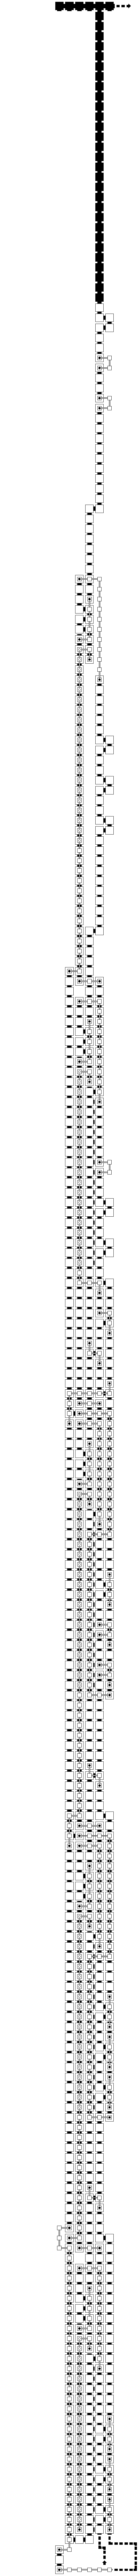
\includegraphics[width=0.45in]{overviews/case3/roof_unit_3_op_msr_msd}}}%
    ~
    \caption{\label{fig:roof_units} The {\roofunit} gadgets.}
\end{figure}